\chapter{แนวคิด ทฤษฎีและงานวิจัยที่เกี่ยวข้อง}
\label{chapter:related-theory}

\section{ระบบให้การแนะนำ (Recommendation System)}
ระบบให้การแนะนำ \cite[baptiste]{baptiste} เป็นระบบสนับสนุนการตัดใจที่จะให้การแนะนำสินค้าหรือบริหารที่มีความเหมาะสมกับรูปแบบและพฤติกรรมของลูกค้าหรือยูสเซอร์แต่ละคน โดยอาศัยข้อมูลของยูสเซอร์งานร่วมกับข้อมูลประกอบภายนอกมาใช้ในการวิเคราะห์คัดกรอง ให้ได้สิ่งที่มีความหมายที่เหมาะสมกับยูสเซอร์งาน โดยมีเทคนิคแบ่งย่อยได้เป็นสองชนิดหลัก ๆ คือ การกรองแบบอิงเนื้อหา (Content Based Filtering) การกรองแบบร่วม (Collaborative Filtering) และการกรองแบบผสม (Hybrid Recognition) \cite{robin}

\begin{figure}[!h]
  \centering
  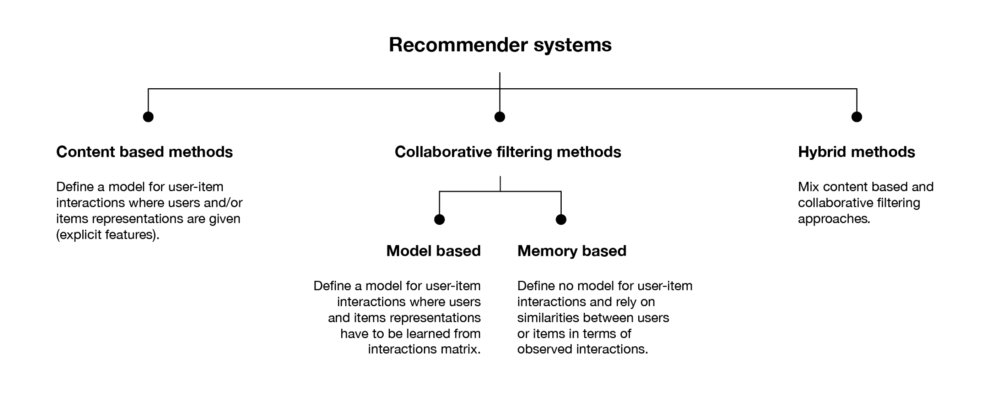
\includegraphics[width=1\textwidth]{colla_content_overall.png}  
  \caption{\cite[baptiste]{baptiste}อัลกอริทึมระบบผู้แนะนำประเภทต่างๆ}
  \label{Fig:colla_content_overall}
\end{figure}

\subsection{การกรองแบบร่วมกัน (Collaborative Filtering)}
\begin{figure}[!h]
  \centering
  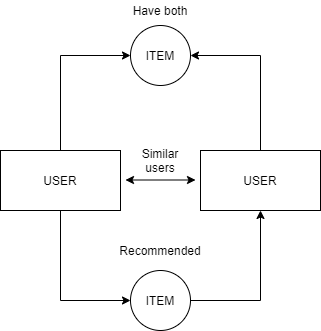
\includegraphics[width=0.4\textwidth]{CF.png}  
  \caption{ภาพรวมการกรองแบบร่วมกัน}
  \label{Fig:cf}
\end{figure}
การกรองแบบร่วม เป็นเทคนิคและนำโดยใช้ข้อมูลการโต้ตอบในอดีตที่ถูกบันทึกไว้ระหว่างยูสเซอร์และรายการเพื่อสร้างคำแนะนำใหม่ ๆ โดยข้อมูลเหล่านี้จะถูกเก็บไว้ในรูปแบบเมทริกซ์ที่เรียกว่า "user-item interactions matrix"
\newline
\begin{figure}[!h]
  \centering
  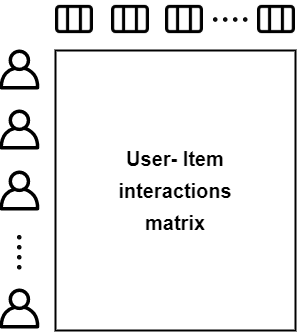
\includegraphics[width=0.3\textwidth]{colla_01.png}  
  \caption{เมทริกซ์การโต้ตอบยูสเซอร์ไอเทม}
  \label{Fig:colla_01}
\end{figure}

แนวคิดหลักที่เป็นกฎของการกรองแบบร่วมกันคือข้อมูลการโต้ตอบในอดีตในประมาณที่มากเพียงพอจะสามารถตรวจหาความคล้ายคลึงกันของยูสเซอร์กับไอเทมหรือยูสเซอร์กับยูสเซอร์ได้ 
คลาสของอัลกอริธึมการกรองแบบร่วมกันแบ่งออกเป็นสองประเภทย่อยที่โดยทั่วไปเรียกว่า อิงจากหน่วยความจำ (memory based) และ อิงจากโมเดล (model based) ในวิธีนี้การทำงานจะไม่มีการสันนิษฐานแบบจำลองแฝงแต่อัลกอริทึมจะทำงานโดยตรงกับข้อมูลการตอบโต้ยูสเซอร์และไอเทม ตัวอย่างเช่น ยูสเซอร์จะแสดงผลลัพธ์ของข้อมูลไอเทมเพื่อนบ้านที่ใกล้เคียงที่สุดเพื่อใช้ในการแนะนำ วิธีนี้จะมีความอคติต่ำในทางทฤษฎีแต่มีความแปรปรวนสูง 
และการอิงจากโมเดล วิธีนี้ถือว่าเป็นรูปแบบปฎิสัมพันธ์แฝง โมเดลนี้จะได้รับการฝึกให้สร้างค่าการตอบโต้ยูสเซอร์ไอเทมใหม่จากการแสดงยูสเซอร์และไอเทมของตัวเอง จากนั้นคำแนะนำใหม่สามารถทำได้โดยใช้โมเดลนี้ การทำนายจะมีความหมายทางคณิตศาสตร์ที่ยากต่อการตีความโดยมนุษย์ ดังนั้นวิธีการนี้ถือว่าเป็นวิธีที่มีความอคติสูงแต่มีความแปรปรวนต่ำ
\newline
\begin{figure}[!h]
  \centering
  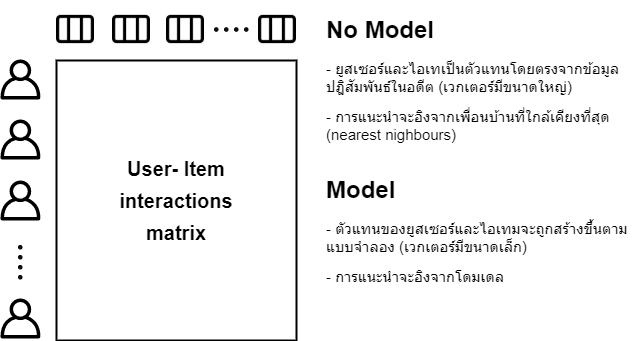
\includegraphics[width=0.8\textwidth]{colla_02.png}  
  \caption{ภาพรวมของกระบวนทัศน์วิธีการกรองร่วมกัน}
  \label{Fig:colla_02}
\end{figure}
\pagebreak

ข้อได้เปรียบหลักของการกรองแบบร่วมกันคือไม่ต้องการข้อมูลเกี่ยวกับยูสเซอร์หรือรายการเป็นตัวตั้งต้น ดังนั้นจึงสามารถใช้ได้ในหลายสถานการณ์ ยิ่งไปกว่านั้นยิ่งข้อมูลการโต้ตอบมีมากขึ้นเท่าใด คำแนะนำใหม่ก็จะยิ่งถูกต้องมากขึ้นเท่านั้น
แต่ถึงอย่างนั้นเนื่องจากไม่ต้องการข้อมูลในการตั้งต้นการพิจารณ์ข้อมูลเพื่อแนะนำจึงเกิดปัญหา นั่นคือ "cold start problem" ในทางปฎิบัติจึงเป็นไปไม่ได้ที่จะแนะนำสิ่งใดให้กับยูสเซอร์ใหม่หรือแนะนำรายการใหม่ให้กับยูสเซอร์ ยูสเซอร์และรายการที่มีข้อมูลการตอบโต้ที่น้อยเกินไปจะทำให้การแนะนำคลาดเคลื่อนเป็นอย่างมาก, ปัญหานี้สามารถแก้ไขได้หลายวิธีอย่างเช่น การแนะนำไอเทมแบบสุ่มให้กับยูสเซอร์ใหม่หรือแนะนำไอเทมใหม่กับยูสเซอร์แบบสุ่ม หรือการแนะนำไอเทมยอดนิยมให้กับยูสเซอร์ใหม่หรือไอเทมใหม่ให้กับยูสเซอร์ส่วนใหญ่ หรือการแนะนำชุดรายการให้กับยูสเซอร์ใหม่หรือรายการใหม่ไปยังกลุ่มยูสเซอร์ที่หลากหลายเป็นต้น

\pagebreak
\subsubsection{Memory Based}
\paragraph{User-user}
ในการแนะนำให้กับยูสเซอร์ วิธี user-user จะพยามระบุผู้ใช้ที่มีข้อมูลโปรไฟล์การโต้ตอบที่คล้ายคลึงกันมากที่สุด (เพื่อนบ้านที่ใกล้ที่สุด) เพื่อแนะนำรายการที่ได้รับความนิยมมากที่สุดให้บรรดาเพื่อนบ้านเหล่านี้ (หมายถึงยูสเซอร์ใหม่) วิธีนี้เรียกว่า "ผู้ใช้เป็นศูนย์กลาง" (user-centered)
สมมติว่าเราต้องการให้คำแนะนำสำหรับยูสเซอร์ใหม่ ขั้นแรกทุกคนจะถูกแทนที่ด้วยเวกเตอร์ของการโต้ตอบกับรายการ หลังจากนั้นเราสามารถคำนวนความคล้ายคลึงกันระหว่างยูสเซอร์ที่เราสนใจกับยูสเซอร์อื่น ๆ ทุกคน การวัดความคล้ายคลึงกันคือการที่ยูสเซอร์สองคนมีปฎิสัมพันธ์คลายคลึงกันในรายการเดียวกันนั่นหมายความว่าควรได้รับการพิจารณาว่าอยู่ใกล้กัน เมื่อคำนวนความคล้ายคลึงกับยูสเซอร์ทุกคนแล้ว เราสามารถเก็บ k nearest neighbour ไว้ให้กับยูสเซอร์ของเราจากนั้นแนะนำรายการที่ได้รับความนิยมมากที่สุดในบรรดารายการเหล่านี้
\newline
\begin{figure}[!h]
  \centering
  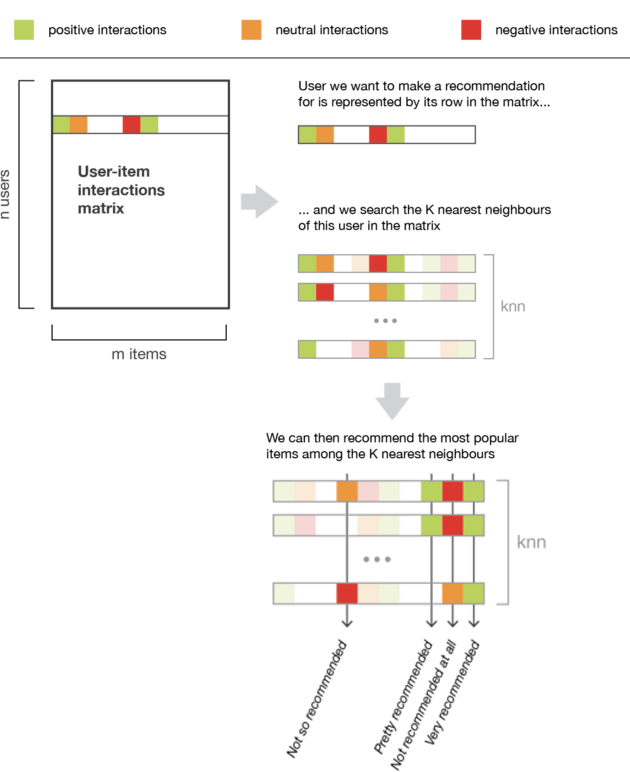
\includegraphics[width=0.8\textwidth]{content_user_user.png}  
  \caption{\cite[baptiste]{baptiste} วิธีการแบบ user-user}
  \label{Fig:content_user_user}
\end{figure}
\paragraph{Item-item}
การให้คะแนะนำใหม่แก่ยูสเซอร์แนวคิดของวิธี item-item คือการหารายการที่สอดคล้องกับรายการที่ยูสเซอร์มีรายการตอบโต้เป็นบวก (position) สองรายการซึ่งจะถือว่าคล้ายกันหากผู้ใช้ส่วนใหญ่ที่มีปฎิสัมพันธ์กับทั้งคู่ทำในลักษณะเดียวกัน วิธีนี้เรียกว่า "item-centered"
\newline
\begin{figure}[!h]
  \centering
  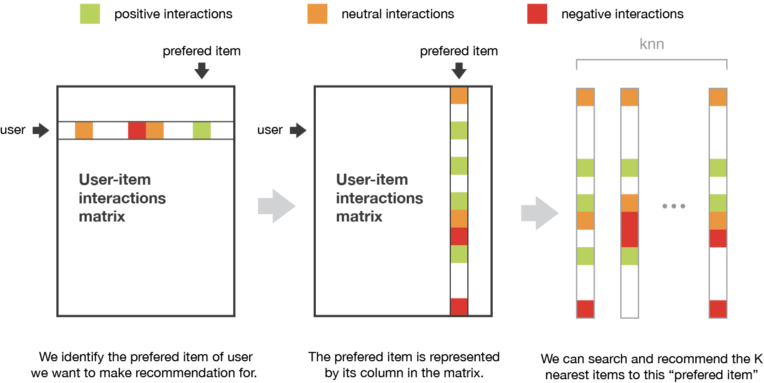
\includegraphics[width=1\textwidth]{content_item_item.png}  
  \caption{\cite[baptiste]{baptiste} วิธีการแบบ item-item}
  \label{Fig:content_item_item}
\end{figure}
\subsubsection{Model Based}
การกรองแบบร่วมกันโดยใช้โมเดล อาศัยข้อมูลการโต้ตอบยูสเซอร์ไอเทม และใช้โมเดลในการอธิบายข้อมูลการโต้ตอบเหล่านี้ ตัวอย่างเช่น อัลกอริธึมการแยกตัวประกอบเมทริกซ์ (matrix factorization) โดยสลายเมทริกซ์การโต้ตอบยูสเซอร์ไอเทมที่มีขนาดใหญ่และกระจายให้ให้เป็นตารางเมทริกซ์ที่มีขนาดเล็กและหนาแน่นจำนวนสองเมทริกซ์
\pagebreak
    

\subsection{การกรองแบบอิงเนื้อหา (Content Based Filtering)}
\begin{figure}[!h]
  \centering
  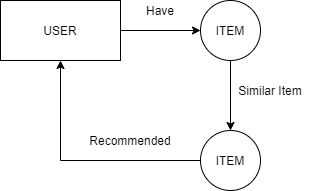
\includegraphics[width=0.4\textwidth]{CB.png}  
  \caption{ภาพรวมการกรองโดยอิงจากเนื้อหา}
  \label{Fig:CB}
\end{figure}
การกรองโดยอิงจากเนื้อหาต่างจากการกรองแแบบร่วมกันที่อาศัยข้อมูลการตอบโต้ยูสเซอร์และไอเทม การกรองโดยอิงจากเนื้อหาใช้ข้อมูลเพิ่มเติมเกี่ยวกับยูสเซอร์ และ/หรือ ไอเทม ยกตัวอย่างเช่นระบบแนะนำภาพยนต์ 
ข้อมูลเพิ่มเติมนี้อาจจะเป็น เพศ, อายุ, งาน หรือข้อมูลส่วนตัวอื่น ๆ ของยูสเซอร์ เพราะฉะนั้นแนวคิดนี้คือการพยามสร้างแบบจำลองตามคุณลักษณะเพื่อพยามอธิบายยูสเซอร์และไอเทม ตัวอย่างเช่น เมื่อพิจารณ์ภาพยนต์ เราจะพยามจำลองความจริงที่ว่าผู้หญิงมักจะให้คะแนนภาพยนต์บางเรื่องตามที่เพศหญิงชอบ และผู้ใช้จะให้คะแนนภาพยนต์บางเรื่องตามที่เพศตัวเองชอบ เป็นต้น หากทำการพิจารณ์จากตัวอย่างข้างต้นเราเพียงแค่ดูโปรไฟล์เพศเราก็สามารถแนะนำภาพยนต์ที่เพศนั้นๆ ชอบได้
\newline
\begin{figure}[!h]
  \centering
  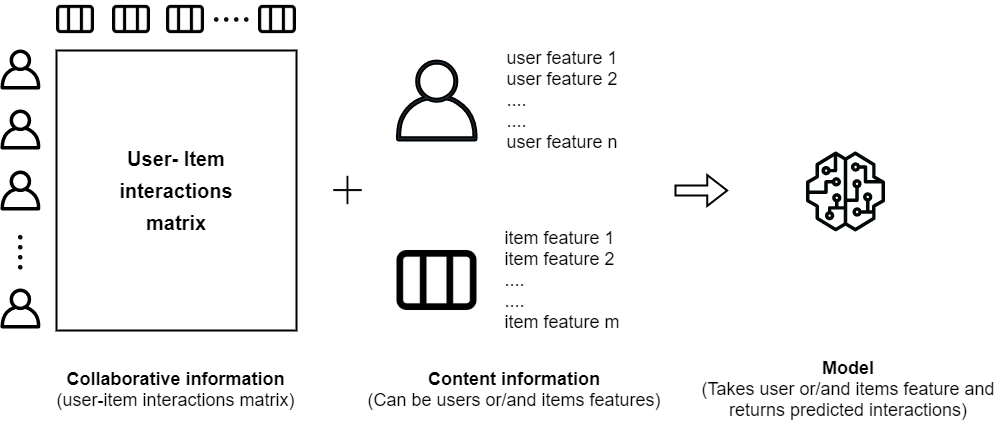
\includegraphics[width=1\textwidth]{content_01.png}  
  \caption{ภาพรวมของกระบวนทัศน์วิธีการกรองโดยอิงจากเนื้อหา}
  \label{Fig:content_01}
\end{figure}
วิธีการอิงจากเนื้อหานั้นไม่จะประสบปัญหา "cold start problem" น้อยกว่าวิธีการอิงแบบร่วมกัน ยูสเซอร์ใหม่หรือไอเทมใหม่สามารถอธิบายได้ตามลักษณะ (เนื้อหา) ของตัวมันเอง และคำแนะนำที่เกี่ยวข้องสามารถทำได้สำหรับเอนทิตีใหม่เหล่านี้ เฉพาะยูสเซอร์ใหม่หรือผู้ใช้ใหม่ที่มีคุณสมบัติที่ไม่เคยเจอมาก่อนเท่านั้นที่ได้รับผลกระทบจากข้อเสียนี้ แต่เมื่อมีข้อมูลมากเพียงพอปัญหานี้จะหมดไป
\pagebreak

\subsection{ระบบให้การแนะนำแบบผสม (Hybrid Recommendation)}
ระบบการแนะนำแบบผสม เป็นการประยุกต์ระบบแนะนำหลายหรือหลายข้อมูลเข้าด้วยกันเพื่อเพิ่มประสิทธิภาพในการทำนาย และแก้ไขปัญหาข้อด้อยของแต่ละเทคนิค


\section{Apache Airflow}
Apache airflow \cite{airflow} เป็นแพลตฟอร์มการจัดการเวิร์กโฟลว์แบบโอเพนซอร์สามารถเขียนโปรแกรมเพื่อกำหนดเวลาขั้นตอนการทำงานและตรวจสอบผ่านอินเทอร์เฟชผู้ใช้ได้
Airflow เขียนด้วยภาษา python และเวิร์กโฟลว์ถูกสร้างผ่านสคริปต์ python โดยได้รับการออกแบบภายใต้หลักการ "configuration as code" แม้ว่าแพลตฟอร์มอื่น ๆ ที่ใช้หลักการนี้จะอยู่ภายใต้มาร์กอัพ เช่น XML แต่การใช้ python ช่วยให้นักพัฒนานำเข้าไลบรารีและคลาสเพื่อช่วยในการสร้างเวิร์กโฟลว์ได้ง่ายและมีประสิทธิภาพมากยิ่งขึ้นกว่าการตั้งค่าโดด ๆ แบบ XML

Airflow ใช้กราฟ acyclic กำกับ (DAG) เพื่อจัดการระเบียบเวิร์ฟเฟลว์งาน และการอ้างอิงถูกกำหนดไว้ใน python จากนั้น airflow จะจัดการตั้งเวลาและดำเนินการ DAG ตามเวลาที่กำหนด (เช่น รายชั่วโมงรายวัน) หรือตามทริกเกอร์เหตุการภายนอก


\section{Docker}
Docker \cite{docker} เป็นเอ็นจิ้นที่มีการทำงานในลักษระจำลองสภาพวแดล้อมขึ้นมาบนเครื่องเซิรฟ์เวอร์เพื่อใช้ในการรันเซอร์วิสที่ต้องการ มีการทำงานคล้ายคลึงกับเครื่องเสมือน (virtual machine) เช่น MVWare, VirtualBox, XEN, KVM แต่ข้อแตกต่างที่ชัดเจนคือ เครื่องเสมือนที่กล่าวมาจำเป็นต้องจำลองทั้งระบบปฎิบัติการ (OS) เพื่อใช้งานและหากต้องการใช้บริการใด ๆ จำเป็นต้องติดตั้งเพิ่มบนระบบปฎิบัติการนั้น แต่สำหรับ docker แล้วจะใช้สิ่งที่เรียกว่าคอนเทนเนอร์ ในการจำลองสภาพแวดล้อมขึ้นมา เพื่อใช้งานสำหรับ 1 บริการ ที่ต้องการใช้งานเท่านั้น โดยไม่ต้องมีส่วนระบบปฎิบัติการเข้าไปเกี่ยวข้องด้วยเหมือนเครื่องเสมือนอื่น ๆ
\newline
\begin{figure}[!h]
  \centering
  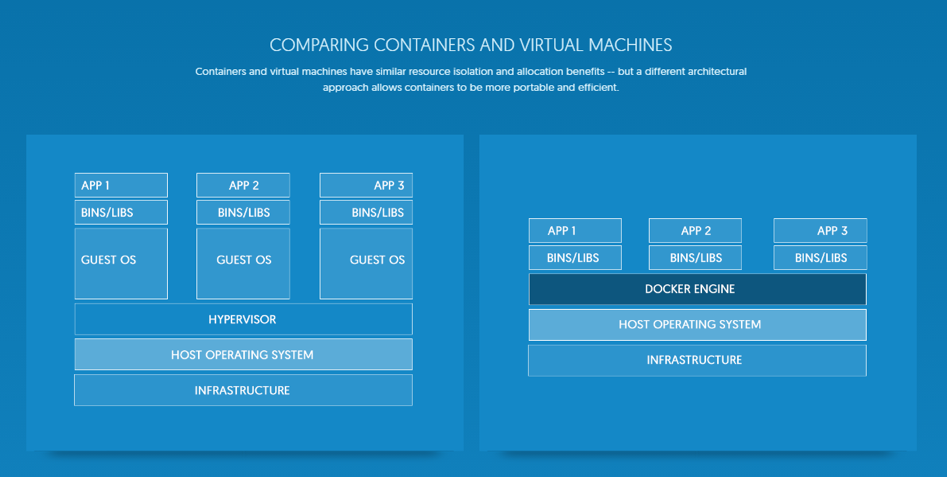
\includegraphics[width=1 \textwidth]{docker.png}  
  \caption{comparing container and virtual machines}
  \label{Fig:docker}
\end{figure}
โดย docker นั้นเป็นที่รู้จักกันอย่างแพร่หลายในช่วง 1-2 ปีที่ผ่านมานี้ เนื่องจากสามารถใช้งานได้อย่างสะดวกและตอบสนองความต้องการของผู้พัฒนาโปรแกรมหรือผู้ดูแลระบบ
\paragraph*{Docker image}
เป็นตัวต้นแบบของคอนเทนเนอร์ซึ่งภายในจะประกอบด้วยแอพพลิเคชั่นต่าง ๆ ที่มีการติดตั้งไว้เพื่อนใช้งานสำหรับบริการนั้น ๆ รวมทั้งมีการตั้งค่าต่าง ๆ ไว้อย่างเรียบร้อย จากนั้นจึงนำมาสร้างเป็นอิมเมจบนรีจิสทรีเพื่อนำมาใช้งานทั้งนี้ผู้ใช้งานสามารถสร้าง docker image ของตัวเองได้อีกด้วย
\paragraph*{Docker container}
เป็นกล่องเหสมือนซึ่งนำ docker image มาติดตั้งเพื่อให้สามารถใช้งานบริการที่ต้องการได้จากอิมเมจนั้น ๆ โดยในคอนเทนเนอร์แต่ละตัวจะมีการใช้งาน RAM, CPU ไฟล์ตั้งค่าต่าง ๆ เป็นของแต่ละคอนเทนเนอร์เอง


\section{การสกัดข้อมูล (Data Scraping)}
การสกัดข้อมูล \cite{choochart} เป็นเทคนิคในการเข้าถึงข้อมูลจากเว็บไซต์เพื่อที่หาและสกัดข้อมูลที่ต้องการ ในการสกัดข้อมูลจากข้อความที่ดึงมาจากเว็บไซต์สามารถใช้ไลบรารี่ beautifulsoup ของภาษา python เพื่อช่วยในการสกัดข้อมูลให้มีความง่ายขึ้นได้ กรณีที่เว็บไซต์ที่ทำงานโดยการเรนเดอร์หน้าเพจทั้งหน้าแล้วส่งมาให้ยูสเซอร์ (client) ราสามารถดึงข้อมูลของทั้งหน้ามาใช้ได้โดยตรงและสกัดข้อมูลจากที่กล่าวมาข้างต้น แต่บางเว็บไซต์ที่มีการทำงานแบบฝั่งไคลเอนต์ มีการแสดงผลข้อมูลเป็นแบบ Asynchronous ซึ่งทำให้ข้อมูลปรากฎขึ้นไม่พร้อมกัน โดยจะขึ้นอยู่กับการกระทำของยูสเซอร์เช่น คลิ๊กเปิด เลื่อนลงเพื่อโหลดฟีด จะไม่สามารถดึงข้อมูลทั้งหน้าได้จำเป็นต้องจำเป็นต้องแก้ปัญหาโดยทำการจำลองบราวเซอร์เพื่อจำลองการกระทำของยูสเซอร์ขึ้นมา
\subsection{Puppeteer}
Puppeteer เป็นไลบรารี่ Node ซึ่งมีอีพีไอระดับสูงเพื่อควบคุม Chrome หรือ Chromium ผ่านหน้าพัฒนา โดย puppeteer จะทำการรันเป็นเบราว์เซอร์ล่องหน (headless browser) หรือคือไม่มีอินเทอร์เฟซผู้ใช้งานแบบกราฟิกโดยเบราว์เซอร์ล่องหนสามารถควบคุมหน้าเว็บได้โดยอัติโนมัติในสภาพแวดล้อมที่คล้ายกับเว็บเบราว์เซอร์ แต่จำเดินการผ่านอินเทอร์เฟซบรรทัดคำสั่งหรือใช้การสื่อสารผ่านเครือข่าย มีประโยชน์เป็นอย่างมากสำหรับการทดสอบหน้าเว็บเนื่องจากสามารถแสดงผลและทำความเข้าใจ HTML ได้อีกทั้งยังสามารถประยุกต์ใช้เบราว์เซอร์ล่องหนในการสกัดข้อมูลจากเว็บไซต์ที่ต้องการผ่านการจำลองเสมือนเพื่อเข้าถึงข้อมูลที่ต้องการ 


\section{การประมวลผลภาษาธรรมชาติ (Natural Language Processing)}
การประมวลผลภาษาธรรมชาติ (NLP) \cite{diego} เป็นแขนงหนึ่งของสาขาปัญญาประดิษฐ์ (Artificial Intelligence) ที่ทำให้เครื่องจักรมีความสามารถในการอ่านทำความเข้าใจและเข้าใจความหมายของภาษามนุษย์ได้ กล่าวคือ NLP แสดงถึงการจัดการภาษามนุษย์โดยอัตโนมัติเช่นการพูด ข้อความ หรือแม้กระทั่งแนวคิดที่สนใจ โดยได้มีการนำไปประยุกต์ใช้ในแขนงมากมายเช่น ช่วยในการทำความเข้าใจและคาดการณ์กลุ่มของยูสเซอร์จากโปรไฟล์ของยูสเซอร์เหล่านั้น เป็นต้น

\subsection{Word Embedding}
Word Embedding \cite{lukkiddd} คือการจับบริบทของคำในเอกสารที่มีความคล้ายคลึงกับคำอื่น ๆ และแปลงคำให้เป็นตัวเลขในรูปแบบเว็กเตอร์ โดยถือเป็นหนึ่งในวิธีการสร้างฟีเจอร์จากคำวิธีหนึ่ง โดยทำการลดขนาดเว็กเตอร์ลงด้วย เช่น ทำการ word embedding กับคำว่า "I, liked, the, hotel" เราจะได้เวกเตอร์ออกมาคือ I[0.3, 0.2, 0.8, 0.1], liked[0.4, 1.2, 0.1, 0.9], the[1.3, -2.1, 0, 1.2], hotel[0.5, 1.4, 0.3, -0.4] เป็นต้น

\subsubsection{Word2Vec}
Word2Vec \cite{lukkiddd} Pre-trained weight model หรือแบบจำลองน้ำหนักที่ผ่านการเทรนมาล่วงหน้าแล้ว word2vec มีสองแบบที่สามารถใช้เพื่อทำ word embeddings คือ CBOW และ Skip-gram
\begin{enumerate}
  \item \textbf{Bag-of-Words Models (CBOW)} โดมเดลนี้จะทำนายคำถัดไปโดยอ้างอิงจาก n คำก่อนหน้าและ n คำต่อท้ายคำถัดไป ตัวอย่างเช่นประโยคต่อไปนี้ 
  
  \centerline{\emph{Lorem ipsum dolor sit amet}}
  
  CBOW จะทำนายคำ \emph{dolar} โดยให้อินพุต n = 2 ก่อนและหลังคำซึ่งจะได้ว่า \emph{Lorem, ipsum, sit} และ \emph{amet} คำเหล่านี้เรียกว่าบริบทของคำเป้าหมายและปริมาณจะเป็นพารามิเตอร์ของแบบจำลอง

  \item \textbf{Skip-gram} จากที่จะคาดเดาตามบริบทของคำ skip-gram จะทำนายบริบทแค่คำเดียว จากตัวอย่างก่อนหน้านี้เมื่อทำการทำนายด้วย skip-gram ตัว skip-gram จะพยามทำนายคำว่า \emph{Lorem, ipsum, sit} และ \emph{amet} โดยมีคำว่า \emph{dolar} เป็นอินพุต
\end{enumerate}

\subsection{Term Frequency-Inverse Document Frequency (TF-IDF)}
TFIDF \cite{cory} ใช้เพื่อชั่งน้ำหนักของคำสำคัญ (Keyword) ในเอกสารใด ๆ เพื่อกำหนดความสำคัญให้กับคำสำคัญเหล่านั้นตามจำนวนครั้งที่ปรากฎในเอกสาร หรือก็คือยิ่งคะแนน TF * IDF(น้ำหนัก) สูงเท่าไหร่คำนั้นก็จะสำคัญเท่านั้น ในทุกคำหรือคำศัพท์แต่ละคำจะมีคะแนน TF และ IDF อยู่เสมอ ผลคูณของคะแนน TF และ IDF ของคำหนึ่งจะเรียกว่าน้ำหนัก TF*IDF ของคำนั้น ๆ
\newline

ความถี่ (TF: Term Frequency) ของคำคือจำนวนครั้งที่ปรากฎในเอกสาร เมื่อทราบถึง TF แล้วเราจะสามารถบอกได้ว่ามีคำนั้นปรากฎในเอกสารบ่อยเท่าใด
\begin{equation}
  TF(t) = \text{จำนวนครั้งที่ } t \text{ ปรากฎบนเอกสาร } / \text{ จำนวนคำทั้งหมดในเอกสาร}
\end{equation}

ความถี่เอกสารผักผัน (IDF: Inverse Document Frequency) ของคำคือการวัดความสำคัญของคำเหล่านั้นในคลังข้อมูลคำ (Copus) ทั้งหมด
\begin{equation}
  IDF(t) = log_e (\text{จำนวนเอกสารทั้งหมด } / \text{ จำนวนเอกสารที่มีคำศัพท์อยู่ในนั้น})
\end{equation}

\begin{equation}
  W_{x, y} = TF_{x, y} \cdot log\left( \frac{N} {DF_{x}} \right)
\end{equation}
\begin{conditions}
  TF_{x, y}     &  frequency of x in y \\
  DF_{x}        &  number of documents containing x \\
  N             &  total number of document
\end{conditions}
เมื่อเราทำ TF-IDF แล้วเราสามารถเห็นความสำคัญของข้อความสำคัญได้


\section{การหาความสอดคล้องระหว่างสองสิ่ง}
ในการหาความสอดคล้องระหว่างสองสิ่ง \cite{selva} เราสามารถทำได้โดยใช้เทคนิคความคล้ายคลึงของโคไซน์ (Cosine Similarity ) 
\newline
\begin{equation}
  sim_{A, B} = \frac{A \cdot B} {||A||||B||} = \frac{\Sigma^{n}_{i=1} A_{i}B_{i}} {\sqrt{\Sigma^{n}_{i=1}A^{2}_{i}} \sqrt{\Sigma^{n}_{i=1}B^{2}_{i}}}
\end{equation}
\newline
ตัวอย่างข้อความ "backend developer", "senior software developer" เมื่อนำมาเปลี่ยนเป็นเมทริกซ์เทคนิคการนับคำ (count vectorizer) จะได้เมทริกซ์ [1, 1, 0, 0] และ [0, 1, 1, 1]
หลังจากมาหาความสอดคล้องจากการแทนค่าจากสมการดังกล่าวจะได้
\newline
\begin{equation}
  sim_{A, B} = \frac{(1\cdot0 + 1\cdot1 + 0\cdot1 + 0\cdot1)} {\sqrt{(1^{2} + 1^{2} + 0^{2} + 0^{2})} \sqrt{(0^{2} + 1^{2} + 1^{2} + 1^{2})}}
\end{equation}
\begin{equation}
  sim_{A, B} = \frac{1} {\sqrt{2} \sqrt{3}}
\end{equation}
ดังนั้นแล้วความสอดคล้องระหว่าง "backend developer" และ "senior software developer" คือ 0.408


\section{Support Vector Machine}
Support Vector Machine (SVG) \cite{cory2} เป็นเทคนิค Pattern Recognition แบบ Supervised Learning ถูกใช้ในเคส Classification และ Regression 
โดยภายในงานนี้ได้ถูกใช้เพื่อ Classification ตำแหน่งงานด้วยการสร้าง Hyper-plane ที่เหมาะสมที่สุด (Optimal)
เพื่อแยกข้อมูลสองกลุ่มด้วย Optimal Hyper-plane นั้น $w \times x - b = 0$ จะทำหน้าที่แบ่งข้อมูลสองกลุ่มออกจากกันด้วยมี Support Vector ทำหน้าที่เป็นกันชนระหว่างข้อมูลที่ใกล้กัน SVM จะสร้างพื้นที่การตัดสินใจขึ้นมา
หรือก็คือพื้นที่ระหว่าง $w \times x - b = 1$ และ $w \times x - b = -1$ โดยจะปรับให้ระยะห่างหรือความกว้างระหว่างทั้งสองนั้นมีค่าสูงที่สุด แต่บางกรณีข้อมูลไม่สามารถแบ่งแยกได้ด้วยเส้นตรง จำเป็นต้องแบ่งข้อมูลแบบ Non-linear ซึ่ง
SVM สามารถใช้ Kernel เข้ามาช่วยในการเปลี่ยนมิติของข้อมูลเพื่อให้สามารถแบ่งแยกข้อมูลทั้งสองกลุ่มได้ด้วย Linear Hyper-plan

\section{เว็บแอพพลิเคชั่น (Web Application)} 
Web Application \cite{margaret} ทำหน้าที่ในการเป็นช่องทางในการเชื่อมต่อระหว่างเว็บไซต์กับผู้ให้บริการไอพีไอจากที่อื่น เป็นตัวกลางที่ทำให้โปรแกรมสามารถประยุกต์เชื่อมต่อกับโปรแกรมประยุกต์อื่น ๆ ได้ เช่น google map ที่ทาง google ให้บริการให้ยูสเซอร์สามารถนำเว็บไซต์ของตนเองเชื่อมต่อกับแผนที่ของ google ได้

\subsection{จาวาสคริปต์ (Javascript)}
เป็นภาษาคอมพิวเตอร์ที่นิยมใช้ในการพัฒนาเว็บแอพพลิชั่น เนื่องจากจาวาสคริปต์มีความสามารถในการจัดการได้ทั้งฝั่งไคลเอนต์ (client) และฝั่งเซิร์ฟเวอร์ (server) ภาษาจาวาสคริปต์เป็นภาษาที่มีคุณสมบัติอะซิงโครนัส (asynchronous) ซึ่งแก้ไขปัญหาการขัดกันระหว่างคำสั่งที่ต้องรอในการรันคำสั่งถัดไปของภาษาที่เป็นซิงโครนัส (synchronous)

\subsection{วิว (Vue)}
Vue.js เป็นไลบรารี่จาวาสคริปต์ที่มุ่งเน้นไปที่เลเยอร์ของมุมมอง(view) สำหรับพัฒนามุมมองผู้ใช้(user interface) โดยในตัวไลบรารี่สามารถรองรับแอพพลิเคชั่นที่ซับซ้อนเช่นระบบ จัดการเส้นทาง(routing) ระบบจัดการสถาณะ(state) และการสร้าง(build)

\section{เอพีไอ (API)}
  Application Programming Interface (API) \cite{wiki api} คือส่วนต่อประสานโปรแรกมประยุกต์ เป็นวิธีการที่ระบบปฎิบัติการ, ไลบรารี และบริการอื่น ๆ เปิดให้โปรแกรมคอมเตอร์สามารถติดต่อเรียกใช้งานได้ โดยเอพีไอสร้างขึ้นจากส่วนสำคัญสองส่วนคือ
  \begin{enumerate}
    \item ข้อกำหนดที่จะอธิบายการแลกเปลี่ยนข้อมูลระหว่างโปรแกรม ที่ทำออกมาในลักษณะของเอกสาร เพื่อว่าคำร้องและการตอบสนองต้องเป็นอย่างไร
    \item ซอฟต์แวร์ที่เขียนขึ้นมาตามข้อกำหนดดังกล่าว และทำการเผยแพร่ออกไปให้ใช้งานได้
  \end{enumerate}
  
  โดยทั่วไปแล้วแอพพลิเคชั่นที่มีเอพีไอจะต้องถูกเขียนเป็นภาษาโปรแกรมมิ่ง และเพื่อการพัฒนาในอนาคต จึงจำเป็นต้องมีการตรวจสอบโครงสร้างของเอพีไอดังนั้น ผู้ออกแบบจึงต้องให้ความสำคัญกับการทดสอบ เพื่อตรวจสอบเงื่อนไขที่สามารถเกิดขึ้นได้จากการใช้งาน

  \subsection*{การใช้งานเอพีไอ} ปัจจุบันเอพีไอถูกใช้งานงานในแอพพลิเคชั่นเพื่อสื่อสารระหว่างไคลเอนต์และเซิร์ฟเวอร์ บริษัทยักใหญ่หลายบริษัทมีการเปิดให้บริการเอพีไอ เพื่อใช้งานภายนอก เช่น twitter, google, facebook โดยใครก็ตามที่สนใจนำบริการเหล่านี้ไปประยุกต์ใช้ สามารถส่งคำร้องเพื่อรับข้อมูลที่ต้องการ หรือถึงส่งคำร้องเพื่อขอบริการได้
    \paragraph*{ไลบรารีและเฟรมเวิร์ค} 
      โดยปกติแล้วเอพีไอ จะเกี่ยวข้องกับไลบรารีซอฟต์แวร์ เอพีไอจำเป็นต้องอธิและข้อกำหนด เอพีไอเดียวสามารถมีการใช้งานได้หลากหลาย (หรือไม่มีเลย) ในรูปแบบของไลบรารี่ต่าง ๆ ที่ใช้อินเทอร์เฟชการเขียนโปรแรกมร่วมกัน การแยกเอพีไอออกจากการนำไปใช้งาน สามารถทำให้โปรแกรมที่เขียนภาษาหนึ่งใช้ไลบรารีที่เขียนด้วยอีกภาษาหนึ่งได้ ตัวอย่างเช่นเนื่องจากภาษา scala และภาษา java คอมไล์เป็น bytecode ที่เข้ากันได้ นักพัฒนา scala จึงสามารถใช้ประโยชน์จากภาษาโปรแกรมที่เกี่ยวข้องกับเอพีไอภาษา Java ได้เป็นต้น \par
    \paragraph*{ระบบปฎิบัติการ}
      เอพีไอสามารถระบุอินเทอร์เฟซระหว่างแอพพลิเคชั่นและระบบปฎิบัติการได้ ตัวอย่างเช่น microsoft ได้สร้างความมุ่งมั่นอย่างยิ่งต่อเอพีไอที่เข้ากันได้กับไลบรารี่ windows api (win32) ดังนั้นแอพพลิเคชั่นรุ่นเก่าอาจทำงานบน windows เวอร์ชั่นใหม่โดยใช้งานตั้งค่าเฉพาะปฎิติบัติการที่เรียกว่า "โหมดความเข้ากัน" เป็นต้น
    \paragraph*{รีโมทเอพีไอ}
      รีโมทเอพีไอถูกใช้ให้นักพัฒนาสามารถเข้าควบคุมทรัพยากรผ่านทางโปรโตคอลเพื่อให้มีมาตราฐานการสือสารเดียวกัน ถึงแม้ว่าจะเป็นคนละเทคโนโลยี เช่น ฐานข้อมูลเอพีไอสามารถอนุญาตให้นักพัฒนาเข้ามาดึงข้อมูลในฐานข้อมูลได้หลากหลายชนิดได้ผ่านฟังค์ชั่นเดียวกัน เพราะฉะนั้นรีโมทเอพีไอจึงถูกใช้บ่อยในงานรักษาด้วยทำทำงานที่ฝั่งไคลเอนต์ให้ไปดึงข้อมูลจากเซิร์ฟเวอร์กลับลงมาทำงาน
    \paragraph*{เว็บเอพีไอ}
      เว็บเอพีถูกใช้กันอย่างแพร่หลายในปัจจุบัน เนื่องจากเป็นเอพีไอที่อยู่ในกลุ่มของ HTTP และขยายออกไปสู่รูปแบบต่าง ๆ เช่น XML และ JSON ซึ่งโดยรวมแล้วจะอยู่บนเว็บเซอร์วิซ เช่น SOUP หรือ REST เป็นต้น

  \subsection*{ตัวอย่างเอพีไอที่นิยมในปัจจุบัน}
    \begin{enumerate}
      \itemsep0em 
      \item \textbf{Google Maps API} เปิดให้ใช้งานเพื่อนำเอาแผนที่ของ Google มาลงใน webpage โดยอาศัย JavaScript หรือ Flash
      \item \textbf{Youtube API} Google ยอมให้ developer สามารถนำเอา Clip video บน YouTube ไปลงใน website หรือ application ได้
      \item \textbf{Flickr API} เพื่อให้ developer สามารถเข้าถึง คลังรูปภาพใน community
      \item \textbf{Twitter API} มี REST API ให้ค้นหา แล้วตรวจสอบข้อมูล trends ได้
      \item \textbf{Amazon product advertising API} เปิด API ให้ใช้ค้นหาสินค้า และ การโฆษณาผ่านทาง website
    \end{enumerate}

  \subsection{Flask}
  เฟลค คือเว็บเฟรมเวิร์คเป็นเฟรมเวิร์คที่เขียนขึ้นมาสำหรับใช้งานในภาษา Python   ไพทอน (ไพธอน)  เพื่อใช้ในการสร้างเว็บไซต์ ทำให้ภาษาไพธอนนั้น มีความสามารถในการจัดการกับเว็บไซต์ซึ่งทำให้มึความสามารถคล้ายๆภาษา PHP (พีเอชพี)  ซึ่งแทบจะใช้แทนกันได้เลย  ในปัจจจุบันมีผู้ใช้ Flask Framework ค่อนข้างจะเยอะมากซึ่งเป็นผลมาจากการใช้งานที่ง่ายและผนวกกับมีผู้ใช้ภาษาไพธอนเพิ่มขึ้นนั่นเอง
    \paragraph*{Python} ภาษาโปรแกรม Python \cite{python} คือภาษาโปรแกรมคอมพิวเตอร์ระดับสูง โดยถูกออกแบบมาให้เป็นภาษาสคริปต์ที่อ่านง่าย  โดยตัดความซับซ้อนของโครงสร้างและไวยกรณ์ของภาษาออกไป ในส่วนของการแปลงชุดคำสั่งที่เราเขียนให้เป็นภาษาเครื่อง Python มีการทำงานแบบ Interpreter คือเป็นการแปลชุดคำสั่งทีละบรรทัด เพื่อป้อนเข้าสู่หน่วยประมวลผลให้คอมพิวเตอร์ทำงานตามที่เราต้องการ นอกจากนั้นภาษาโปรแกรม Python ยังสามารถนำไปใช้ในการเขียนโปรแกรมได้หลากหลายประเภท โดยไม่ได้จำกัดอยู่ที่งานเฉพาะทางใดทางหนึ่ง (General-purpose language) จึงทำให้มีการนำไปใช้กันแพร่หลายในหลายองค์กรใหญ่ระดับโลก เช่น Google, YouTube, Instagram, Dropbox และ NASA เป็นต้น 

% \section{กระบวนการวัด (Measurement Process)}
% การวัดผลซอฟต์แวร์มีบทบาทสำคัญในกิจกรรมการพัฒนาซอฟต์แวร์ทั้งหมด พอลกู๊ดแมนผู้เขียนแนวทางปฏิบัติของเมตริกซอฟต์แวร์อ้างว่าบทบาทของเมตริกซอฟต์แวร์คือการช่วยให้วิศวกรและผู้จัดการสามารถอยู่รอดได้ในสภาพแวดล้อมทางธุรกิจในปัจจุบัน \cite[paul goodman]{paul} การวัดที่ได้มาจากการวัดผลคือตัวเลขที่ใช้ในการสร้างเมตริกและเมตริกคือตัวเลขที่เปลี่ยนเป็นข้อมูล ผู้จัดการจำเป็นต้องมีพื้นฐานในการประเมินคุณภาพผลิตภัณฑ์และวิเคราะห์ประเด็นหรือปัญหาและเป็นพื้นฐานสำหรับการควบคุมเชิงปริมาณของกระบวนการจัดการโครงการและวิศวกรรม นอกจากนี้การวัดผลยังให้ข้อมูลเชิงลึกที่ผู้จัดการต้องใช้ในการตัดสินใจที่สำคัญต่อความสำเร็จของโครงการ \cite[PSM Group]{psm group} โปรแกรมการวัดผลที่มีประสิทธิภาพช่วยและทำให้พวกเขาประสบความสำเร็จโดยการพัฒนาแผนการที่ทำได้
% \subsection{Planning}